\documentclass[11pt,aspectratio=169]{beamer}

% -------------------- THEME & LAYOUT --------------------
\usetheme{Madrid}
\usecolortheme{dolphin} % base color scheme
\usefonttheme{professionalfonts}
\setbeamercovered{transparent}
\setbeamertemplate{navigation symbols}{}   % remove navigation buttons
\setbeamertemplate{caption}[numbered]      % numbered captions
\setbeamertemplate{itemize items}[triangle]
\setbeamersize{text margin left=1.2cm,text margin right=1.2cm} % adjust to taste

% -------------------- GLOBAL FONT SETTINGS --------------------

% 1. Force the base beamer font to small
\setbeamerfont{normal text}{size=\small}

% 2. Force math environments to follow the "small" font size
\setbeamerfont{math text}{size=\small}
\setbeamerfont{equation}{size=\small}

% 3. Redefine \normalsize itself 
% This ensures equations and lists (which look for \normalsize) use  instead.
\let\oldnormalsize\normalsize
\renewcommand{\normalsize}{\oldnormalsize\small}

% 4. Ensure lists also stay small
\setbeamerfont{itemize/enumerate body}{size=\small}
\setbeamerfont{itemize/enumerate subbody}{size=\small}


% -------------------- FONTS & TYPOGRAPHY --------------------
\usepackage[T1]{fontenc}
\usepackage[utf8]{inputenc}
\usepackage{newpxtext,newpxmath} % Palatino-like font & math
\usepackage{microtype}

% -------------------- MATH, TABLES & GRAPHICS --------------------
\usepackage{amsmath,amssymb,amsfonts,mathtools}
\usepackage{bm,booktabs,siunitx,graphicx}
\graphicspath{{./}{./figures/}}
\renewcommand{\theequation}{6.\arabic{equation}}
\renewcommand{\thefigure}{\thechapter.\arabic{figure}} % 6.1, 6.2, etc.
% -------------------- UTILITIES --------------------
\usepackage{appendixnumberbeamer}
\usepackage{ragged2e}
\usepackage{xspace}
\usepackage{csquotes}
% -------------------- Bibliography --------------------
\usepackage[backend=biber,style=authoryear]{biblatex}
\addbibresource{sources.bib}
\usepackage{xcolor}

% -------------------- HYPERREF --------------------
\hypersetup{
  colorlinks=false,
  pdfauthor={Francesca},
  pdftitle={Chapter 1 — The Value of Currency}
}

% -------------------- COLORS & EMPHASIS --------------------
\definecolor{myblue}{RGB}{0,70,140}
\definecolor{myred}{RGB}{180,30,30}
\definecolor{mygreen}{RGB}{0,120,70}
\definecolor{gold}{RGB}{184,134,11}

\setbeamercolor{title}{fg=gold}       % title page
\setbeamercolor{frametitle}{fg=gold}  % slide titles
\setbeamercolor{structure}{fg=gold}   % bullets, sections, links
\setbeamercolor{section in head/foot}{fg=gold,bg=black!10} % gold text on light background

% -------------------- FOOTLINE --------------------
\setbeamertemplate{footline}{
  \leavevmode%
  \hbox{%
    % Section links (hidden if no current section)
    \begin{beamercolorbox}[wd=0.7\paperwidth,ht=2.5ex,dp=1.5ex,leftskip=1.4em]{section in head/foot}%
      \ifx\insertsection\empty
        % nothing
      \else
        Section: \insertsection
      \fi
    \end{beamercolorbox}%
    % Frame number right
    \begin{beamercolorbox}[wd=0.3\paperwidth,ht=2.5ex,dp=1.5ex,leftskip=3.8cm]{section in head/foot}%
      \insertframenumber/\inserttotalframenumber
    \end{beamercolorbox}%
  }%
  \vskip1pt%
}



\newcommand{\highlight}[1]{\textcolor{myblue}{#1}}
\newcommand{\warning}[1]{\textcolor{myred}{#1}}

% -------------------- SHORTCUTS --------------------
\newcommand{\E}{\mathbb{E}}
\newcommand{\R}{\mathbb{R}}
\newcommand{\dd}{\mathrm{d}}
\newcommand{\mc}[1]{\mathcal{#1}}
\newcommand{\bb}[1]{\mathbb{#1}}
\newcommand{\uc}{U_c}
\newcommand{\zg}{Z_g}

% -------------------- TIGHTER DISPLAY MATH --------------------
\makeatletter
\g@addto@macro\normalsize{%
  \setlength\abovedisplayskip{8pt}%
  \setlength\belowdisplayskip{8pt}%
  \setlength\abovedisplayshortskip{6pt}%
  \setlength\belowdisplayshortskip{6pt}%
}
\makeatother
\setbeamertemplate{frametitle}{
  \nointerlineskip
  \begin{beamercolorbox}[wd=\paperwidth,ht=3.5ex,dp=1ex,center]{frametitle}
    \centering\insertframetitle
  \end{beamercolorbox}
}

% -------------------- METADATA --------------------
\title[Part I — Currency and Money]{\textbf{Part I: Currency and Money}\\[2pt]\large Chapter 1 — The Value of Currency}
\subtitle{Currency, Money, and Price-Level Determination}
\author{Francesca}
\institute{}
\date{\today}

% -------------------- SECTION ROADMAP --------------------
\AtBeginSection[]
{
  \begin{frame}
    \tableofcontents[currentsection, hideothersubsections]
  \end{frame}
}


\begin{document}
\setcounter{equation}{0}


% ===================== TITLE SLIDE =====================
\begin{frame}[plain] % 'plain' removes header/footer for the title slide

\begin{columns}[T,totalwidth=\textwidth]

% ----- Left column: Main title, professor, chapter -----
\begin{column}{0.45\textwidth}
\vspace{2cm}

% Main title
{\usebeamercolor[fg]{title}\LARGE\textbf{Monetary Economics}\\[0.3cm]
\LARGE\textbf{and Policy}} 

\vspace{0.5cm}

% Professor name and date
{\large\textit{Pierpaolo Benigno}}\\[0.1cm]

\vspace{1cm}

% Chapter and subtitle
{\usebeamercolor[fg]{frametitle}\large Chapter 6: An AS-AD Graphical Analysis}

\end{column}

% ----- Right column: Image -----
\begin{column}{0.55\textwidth}
\vspace{1cm}
\centering
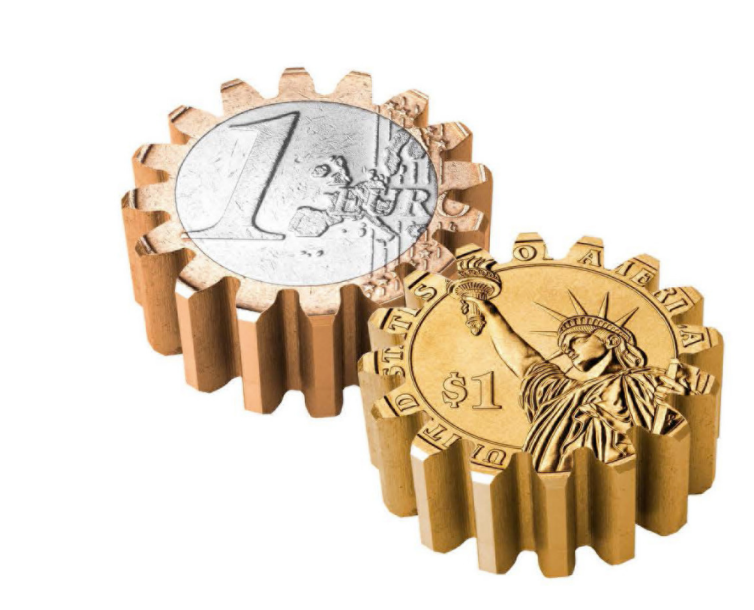
\includegraphics[width=0.9\linewidth]{Cover.png}
\end{column}

\end{columns}

% ----- Footer text (bottom-right corner) -----
\vspace*{2cm} % adjust if needed
\hfill{\large\textit{Prepared by Marcos Consuegra}}

\end{frame}


\begin{frame}{What We Will We Learn}
\small

\begin{itemize}


\item We derive simplified expressions for the \textbf{Aggregate Demand} and \textbf{Aggregate Supply} equations of the New-Keynesian Model, highlighting their slopes, intuition, and policy shifters.

\vspace{0.25cm}

\item We introduce the \textbf{frictionless (Wicksellian) real interest rate} $r_t^{e}$ and use it to interpret monetary policy stabilization in terms of price stability and output-gap elimination.

\vspace{0.25cm}

\item We analyze how different shocks—\textbf{productivity, markup, fiscal, preference, and expectation shocks}—shift AD and AS differently, producing or eliminating policy trade-offs.

\vspace{0.25cm}

\item We identify when monetary policy can jointly stabilize inflation and the output gap, and when it faces an unavoidable \textbf{trade-off}.

\end{itemize}

\end{frame}


% OUTLINE
\begin{frame}{Outline}
\tableofcontents
\end{frame}




\section{Introduction}

% --- SLIDE: The Two Core Equations of the NK Model ---
\begin{frame}{The Two Core Equations of the New Keynesian Model}
\small

\textbf{1. New Keynesian Aggregate Supply (NK Phillips Curve)}
\[
\pi_t - \pi
=
\kappa\,(\hat{Y}_t - \hat{Y}_t^n)
+
\beta\, E_t(\pi_{t+1}-\pi),
\]
where:
\[
\kappa = 
\frac{1-\alpha}{\alpha}
\frac{(1-\alpha\beta)(\sigma^{-1}+\eta)}{1+\theta\eta}.
\]

\begin{itemize}
    \item Inflation increases with the \textbf{output gap}.
    \item Future output gaps and expected inflation affect current inflation.
    \item Sticky prices ($\alpha>0$) $\rightarrow$ \textbf{AS is upward sloping}.
\end{itemize}

\end{frame}

% --- SLIDE: Forward-Looking Aggregate Demand Equation ---
\begin{frame}{The Two Core Equations of the New Keynesian Model}
\small

\textbf{2. New Keynesian Aggregate Demand (IS Equation)}
\[
\hat{Y}_t =
\hat{G}_t
+
E_t(\hat{Y}_{t+1}-\hat{G}_{t+1})
-
\sigma\!\left[
\hat{\imath}_t - E_t(\pi_{t+1}-\pi)
+ E_t(\hat{\xi}_{t+1}-\hat{\xi}_t)
\right].
\]

\begin{itemize}
    \item Output depends negatively on the \textbf{real interest rate}.
    \item Expectations about future rates affect output \emph{today}.
    \item Fiscal demand and preference shocks shift $AD$ directly.
\end{itemize}

\end{frame}


%==================================================
\begin{frame}[label=ASADIntro]{AS–AD Framework: Simplifying Assumptions}
\small

\textbf{Assumptions:}
\begin{itemize}
\item \textbf{Two-period} perfect-foresight economy: short run $t$, long run $t+1$.
\item In the long run, prices are fully flexible and output equals the natural level:
\begin{equation*}
\hat{Y}_{t+1} = \hat{Y}_{t+1}^{n}.
\end{equation*}
\item Policy anchors the long-run price level:
\begin{equation*}
p_{t+1} = p^{*}.
\end{equation*}
\end{itemize}

\textbf{Normalizations:}
\begin{itemize}
\item Inflation target set to zero: $\pi = 0$.
\item Initial price level fixed at the long-run anchor:
\begin{equation*}
p_{t-1} = p^{*}.
\end{equation*}
\end{itemize}

\end{frame}


% --- SLIDE: Deriving the Simple AD Equation from the NK IS Equation ---
\begin{frame}{From NK IS Equation to the AD Representation}
\small

\textbf{Starting point: NK Aggregate Demand (IS Equation)}
\[
\hat{Y}_t =
\hat{G}_t +
E_t(\hat{Y}_{t+1}-\hat{G}_{t+1})
-
\sigma\!\left[
\hat{\imath}_t - E_t(\pi_{t+1}-\pi)
+ E_t(\hat{\xi}_{t+1}-\hat{\xi}_t)
\right].
\]

\vspace{0.25cm}

\textbf{Step 1: Perfect-foresight assumption}
\[
E_t(\hat{Y}_{t+1}) = \hat{Y}_{t+1}, 
\qquad 
E_t(\hat{G}_{t+1}) = \hat{G}_{t+1},
\qquad
E_t(\hat{\xi}_{t+1}) = \hat{\xi}_{t+1}.
\]

\vspace{0.25cm}

\textbf{Step 2: Long-run equilibrium conditions}
\[
\underbrace{\hat{Y}_{t+1}}_{\text{future output}}
=
\underbrace{\hat{Y}_{t+1}^{n}}_{\text{natural level}},
\qquad
\underbrace{\pi_{t+1}}_{\text{future inflation}}
=
p_{t+1}-p_t
=
\underbrace{p^{\ast} - p_t}_{\text{price-level anchor}}.
\]

\vspace{0.25cm}

\textbf{Step 3: Substitute into NK IS and simplify}
\[
\hat{Y}_t
=
\hat{G}_t
+
(\hat{Y}_{t+1}^{n} - \hat{G}_{t+1})
-
\sigma\!
\left[
\hat{\imath}_t 
+ 
(p_t - p^{\ast})
+
(\hat{\xi}_{t+1}-\hat{\xi}_t)
\right].
\]

\end{frame}


%==================================================
\begin{frame}[label=ADRelation]{AD Equation: Short-Run Relationship}
\small

\textbf{AD Equation under Perfect Foresight:}
\begin{equation}
\hat{Y}_{t}=\hat{G}_{t}+\hat{Y}_{t+1}^{n}-\hat{G}_{t+1}-\sigma \left( 
\hat{\imath}_{t}+p_{t}-p^{\ast }+\hat{\xi}_{t+1}-\hat{\xi}_{t}\right)
\label{ADsimple}
\end{equation}

\textbf{Properties:}
\begin{itemize}
\item Negative short-run relationship between output $\hat{Y}_{t}$ and price level $p_{t}$ $\Bigl( \frac{\partial \hat{Y}_t}{\partial p_t}=-\sigma\Bigr)$.
\item  Higher $p_t$ raises the real interest rate $\Rightarrow$ postponing consumption $\Rightarrow$ $\hat{Y}_t\downarrow$.
\item Figure 1 illustrates the downward-sloping schedule.
\end{itemize}

\textbf{AD Shifters:}
\begin{itemize}
\item Exogenous shocks: $\hat{G}_{t}$, $\hat{G}_{t+1}$, $\hat{\xi}_{t}$, $\hat{\xi}_{t+1}$.
\item Long-run changes in natural output: $\hat{Y}_{t+1}^{n}$.
\item Monetary policy shifts via $\hat{\imath}_{t}$ and long-run price target $p^{\ast}$.
\end{itemize}
\end{frame}

% --- SLIDE: From NKPC to the Short-Run AS Curve ---
\begin{frame}{From NKPC to the Short-Run Aggregate Supply Curve}
\small

\textbf{Starting point: New Keynesian Phillips Curve}
\[
\pi_t - \pi
=
\kappa(\hat{Y}_t - \hat{Y}_t^{n})
+
\beta\, E_t(\pi_{t+1}-\pi).
\]

\vspace{0.25cm}

\textbf{Step 1: Perfect-foresight, two-period setting}
\[
E_t(\pi_{t+1}) = \pi_{t+1}, 
\qquad 
\pi_t = p_t - p_{t-1},
\qquad 
\pi_{t+1} = p_{t+1} - p_t.
\]

\textbf{Step 2: Long-run anchors and inflation target}
\[
p_{t+1} = p^{\ast}, 
\qquad 
p_{t-1} = p^{\ast},
\qquad 
\pi = 0.
\]

\vspace{0.25cm}

\textbf{Substitute into NKPC:}
\[
p_t - p^{\ast}
=
\kappa(\hat{Y}_t - \hat{Y}_t^{n})
+
\beta (p^{\ast} - p_t).
\]

\textbf{Short-run AS relationship:}
\[
p_t - p^{\ast}
=
\frac{\kappa}{1+\beta}\,(\hat{Y}_t - \hat{Y}_t^{n}).
\]

\end{frame}

\begin{frame}[label=ASRelation]{AS Equation: Short-Run Relationship}
\small

\textbf{AS Equation under Perfect Foresight:}
\begin{equation}
p_{t}-p^{\ast }=\frac{\kappa}{1+\beta}(\hat{Y}_{t}-\hat{Y}_{t}^{n})
\label{ASsimple}
\end{equation}

\textbf{Properties:}
\begin{itemize}
\item Positive short-run relationship between price level $p_{t}$ and output $\hat{Y}_{t}$ $\Bigl(\frac{\partial p_t}{\partial \hat{Y}_t}=\frac{\kappa}{1+\beta}\Bigr)$.
\item Higher output increases marginal costs, driving prices upward.
\item Figure 1 depicts the upward-sloping curve. Note that the $AS$ passes through $\hat{Y}_t = \hat{Y}_t^n$ and $p_t = p^{\ast}$.
\end{itemize}

\textbf{AS Shifters:}
\begin{itemize}
\item Only short-run shocks affecting the natural level $\hat{Y}_{t}^{n}$ shift the schedule (e.g., via productivity, government spending and markup shocks).
\item Long-run monetary policy modifies $p^{\ast}$ but leaves $p_{t-1}$ unaffected.
\end{itemize}
\end{frame}

\begin{frame}{Baseline Equilibrium}
    % changed [T] to [c] for vertical centering
    \begin{columns}[c] 
    
        \begin{column}{0.35\textwidth}
            \small
            \textbf{Short-Run Equilibrium $E$:}
            \begin{itemize}
                \item Intersection of $AD$ \eqref{ADsimple} and $AS$ \eqref{ASsimple}.
                \item $AS$ equation passes through $\hat{Y}_t = \hat{Y}_t^n$ and $p_t = p^{\ast}$.
            \end{itemize}
        \end{column}

        \begin{column}{0.6\textwidth}
            \centering
            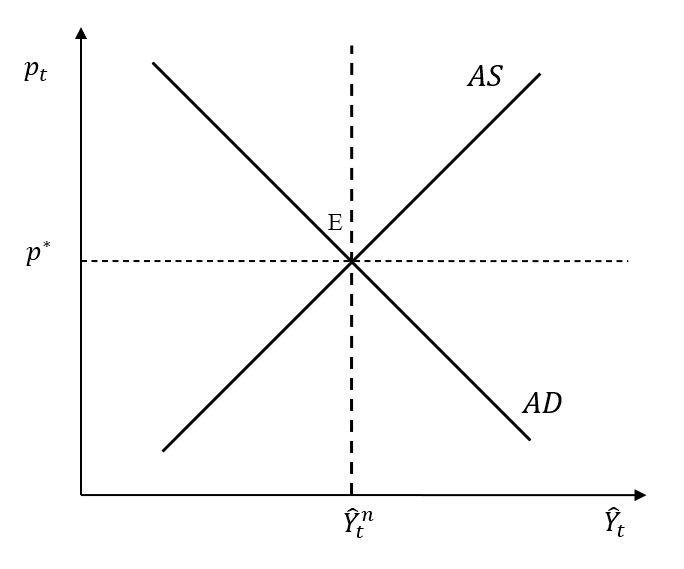
\includegraphics[width=\linewidth]{Figures/Figure3.png}
        \end{column}
    \end{columns}
\end{frame}

%==================================================
%==================================================
\begin{frame}{Natural and Efficient Output: Short and Long Run}
\small

% Use a single align environment for perfect vertical alignment
\textbf{Short run ($t$):}
\begin{align}
\hat{Y}^{e}_{t} &= \frac{1+\eta}{\sigma^{-1}+\eta} \hat{A}_t
                 + \frac{\sigma^{-1}}{\sigma^{-1}+\eta} \hat{G}_t, \label{Efficient1} \\
\hat{Y}^{n}_{t} &= \frac{1+\eta}{\sigma^{-1}+\eta} \hat{A}_t
                 + \frac{\sigma^{-1}}{\sigma^{-1}+\eta} \hat{G}_t
                 - \frac{1}{\sigma^{-1}+\eta} \hat{\mu}_t, \label{Natural1} \\
\end{align}
\textbf{Long run ($t+1$):}
\begin{align}
\hat{Y}^{e}_{t+1} &= \frac{1+\eta}{\sigma^{-1}+\eta} \hat{A}_{t+1}
                   + \frac{\sigma^{-1}}{\sigma^{-1}+\eta} \hat{G}_{t+1}, \label{Efficient2} \\
\hat{Y}^{n}_{t+1} &= \frac{1+\eta}{\sigma^{-1}+\eta} \hat{A}_{t+1}
                   + \frac{\sigma^{-1}}{\sigma^{-1}+\eta} \hat{G}_{t+1}
                   - \frac{1}{\sigma^{-1}+\eta} \hat{\mu}_{t+1}. \label{Natural2}
\end{align}

\vspace{0cm} % Pull the bullets up slightly

\begin{itemize}
    \item $\eta > 0$: inverse Frisch elasticity; $\sigma > 0$: IES.
    \item Assumption: $\hat{Y}^{n}_{t+1} = \hat{Y}^{e}_{t+1}$ (by setting $\hat{\mu}_{t+1} = 0$ inefficient shocks are transitory).
\end{itemize}

\end{frame}
%==================================================
%==================================================
%==================================================
%==================================================
\begin{frame}{Frictionless Real Rate of Interest}
\small

\textbf{Concept}
\begin{itemize}
    \item The \emph{frictionless real rate} $r_t^{e}$ is the real interest rate
          consistent with \textbf{price stability} ($p_t = p^{\ast}$)
          and with achieving the \textbf{efficient level of output} in the short run.
    \item It is driven by efficient (non-distortionary) shocks: productivity, public spending, and preference shocks.
\end{itemize}

\vspace{0.25cm}

\textbf{Frictionless real rate of interest}
\[
r^e_t =
\frac{1}{\sigma}
\Big(\hat{Y}^e_{t+1}-\hat{Y}^e_t - (\hat{G}_{t+1}-\hat{G}_t)\Big)
+ (\hat{\xi}_t - \hat{\xi}_{t+1}).
\]

\vspace{0.2cm}

\textbf{AD equation in terms of $r_t^{e}$}
\[
\hat{Y}_t - \hat{Y}_t^{e}
=
-\sigma\left(\hat{\imath}_t - (p^{\ast}-p_t) - r_t^{e}\right).
\]

\begin{itemize}
    \item If the real rate satisfies  
          $\hat{\imath}_t - (p^{\ast}-p_t)=r_t^{e}$,  
          the economy attains efficient output and stable prices.
    \item This is the essence of the \textbf{Wicksellian policy principle}.
\end{itemize}

\end{frame}


%==================================================
\begin{frame}{Frictionless Real Rate of Interest}
\small

\textbf{Equivalent expression in primitive shocks}
\begin{equation}
r_t^{e}
=
\frac{1+\eta}{1+\sigma\eta}\,(\hat{A}_{t+1}-\hat{A}_t)
-
\frac{\eta}{1+\sigma\eta}\,(\hat{G}_{t+1}-\hat{G}_t)
-
(\hat{\xi}_{t+1}-\hat{\xi}_t).
\label{efficientr}
\end{equation}

\textbf{Implications}
\begin{itemize}
    \item \textbf{Productivity improvements} $\Rightarrow r_t^{e}$ rises.  
          Efficient output grows faster → desired consumption smoothing shifts demand forward.

    \item \textbf{Government spending increases} (future vs. today)  
          affect $r_t^{e}$ through wealth and labor-supply channels.

    \item \textbf{Preference shocks} shift $r_t^{e}$ through intertemporal demand for consumption.
\end{itemize}

\vspace{0.2cm}

\textbf{Policy Insight}
\begin{itemize}
    \item $r_t^{e}$ is the real rate that the central bank would implement  
          to keep inflation at target \emph{and} maintain efficient output.
    \item Related modern concept: \textbf{R-star} commonly used by central banks.
\end{itemize}

\end{frame}

%==================================================

%==================================================
\section{Outline of the Results}
\begin{frame}{Outline of the Results}
\small

\begin{itemize}
\item Under \textbf{efficient shocks} (productivity, public spending), \textbf{no policy trade-off} arises: stabilizing prices and the efficient output gap is jointly attainable.
\item The \textbf{required interest rate adjustment} depends on the shock type:
\begin{itemize}
\item temporary vs.\ permanent shocks,
\item news about future shocks.
\end{itemize}
\item Fluctuations in the \textbf{frictionless interest rate} $r_t^e$ serve as an anchor for policy guidance.
\item \textbf{Inefficient shocks} (e.g.\ markup shocks) generate a policy \textbf{trade-off}, and $r_t^e$ can no longer serve as the sole reference for the policy rate.
\end{itemize}
\end{frame}
%==================================================
\section{Productivity Shocks}
% --- SLIDE 1: Temporary Productivity Shock (Setup + Figure) ---
\begin{frame}[label=TempProdSetup]{Temporary Productivity Shock}
\small
\begin{columns}[c]

\begin{column}{0.37\textwidth}
\small
\textbf{Scenario:} A temporary productivity increase at $t$: ($\hat{A}_t \uparrow$).
\\ \vspace{0.3cm}
\textbf{Implications:}
\begin{itemize}
    \item $\hat{Y}_t^{n}\uparrow$, see \eqref{Natural1}.
    \item \textbf{AS shifts downward to AS'}: Higher $\hat{A}_t$ reduces real marginal costs; adjusting firms lower prices.
    \item Equilibrium $E'$ is reached along the \textbf{AD}: A decrease in short-run prices lowers real interest rate, and raises consumption.
\end{itemize}
\end{column}

\begin{column}{0.6\textwidth}
\centering
% Wrapped in figure to allow proper labeling if caption is added later
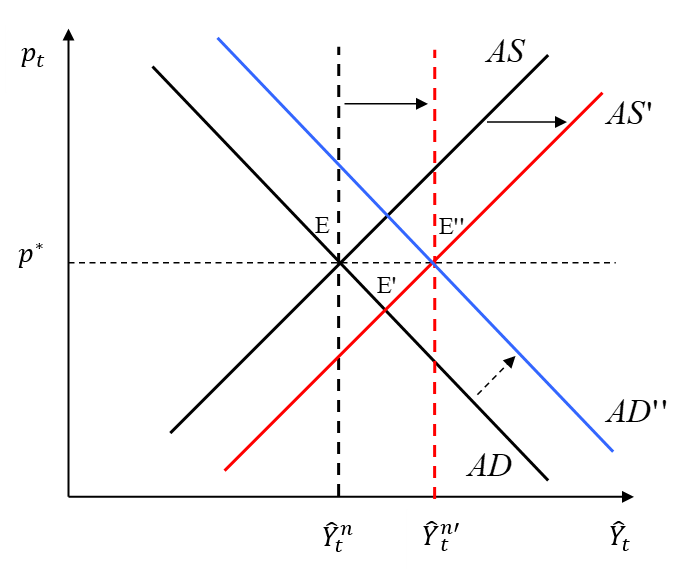
\includegraphics[width=\linewidth]{Figures/Figure4.png}
\label{FigureASAD2} 
\end{column}

\end{columns}
\end{frame}

% --- SLIDE 2: Adjustment Dynamics (E -> E' -> E'') ---
\begin{frame}[label=TempProdDynamics]{Monetary Policy Response}
\small

Without intervention, \textbf{equilibrium ($E'$)} is reached.
\begin{itemize}
    \item Price level is below initial equilibrium, output is higher but remains below the efficient and natural levels; output gap is negative.
    \item Note that efficient and natural output increase in the same proportion.
\end{itemize}

Achieving \textbf{equilibrium ($E''$)} with price stability and closing the output gap:
\begin{itemize}
    \item A lower nominal rate $\hat{\imath}_t$ shifts $AD$ upward to $AD''$.
    \item The new intersection $E''$ features both $p_t = p^{\ast}$ and $\hat{Y}_t = \hat{Y}^n_t = \hat{Y}^e_t$.
\end{itemize}

\textbf{Wicksell interpretation:}
\begin{itemize}
    \item The productivity shock decreases the frictionless real rate $r^e_t$, see \eqref{efficientr}.
    \item The policy rate must fall to track $r^e_t$ to achieve price stability and eliminate the negative output gap.
\end{itemize}
\end{frame}

%==================================================
% --- SLIDE 1: Permanent Productivity Shock (Setup + Figure) ---
\begin{frame}[label=PermProdSetup]{Permanent Productivity Shock}
\small
\begin{columns}[c]

\begin{column}{0.4\textwidth}
\small
\textbf{Scenario:}
\begin{itemize}
    \item Permanent increase in productivity: $\hat{A}_{t} \uparrow$ and $\hat{A}_{t+1} \uparrow$ $\Rightarrow$ $\hat{Y}_{t}^{n}$ and $\hat{Y}_{t+1}^{n}$ $\uparrow$.
\end{itemize}

\textbf{Implications:}
\begin{itemize}
    \item \textbf{AS shifts downwards to AS'}: Lower marginal costs (same as temporary shock).
    \item \textbf{AD shifts upwards to AD'}: $\hat{Y}_{t+1}^{n}$ rises. Households anticipate higher future income and smooth consumption by increasing demand today.
 
\end{itemize}
\end{column}

\begin{column}{0.58\textwidth}
\centering
\begin{figure}
    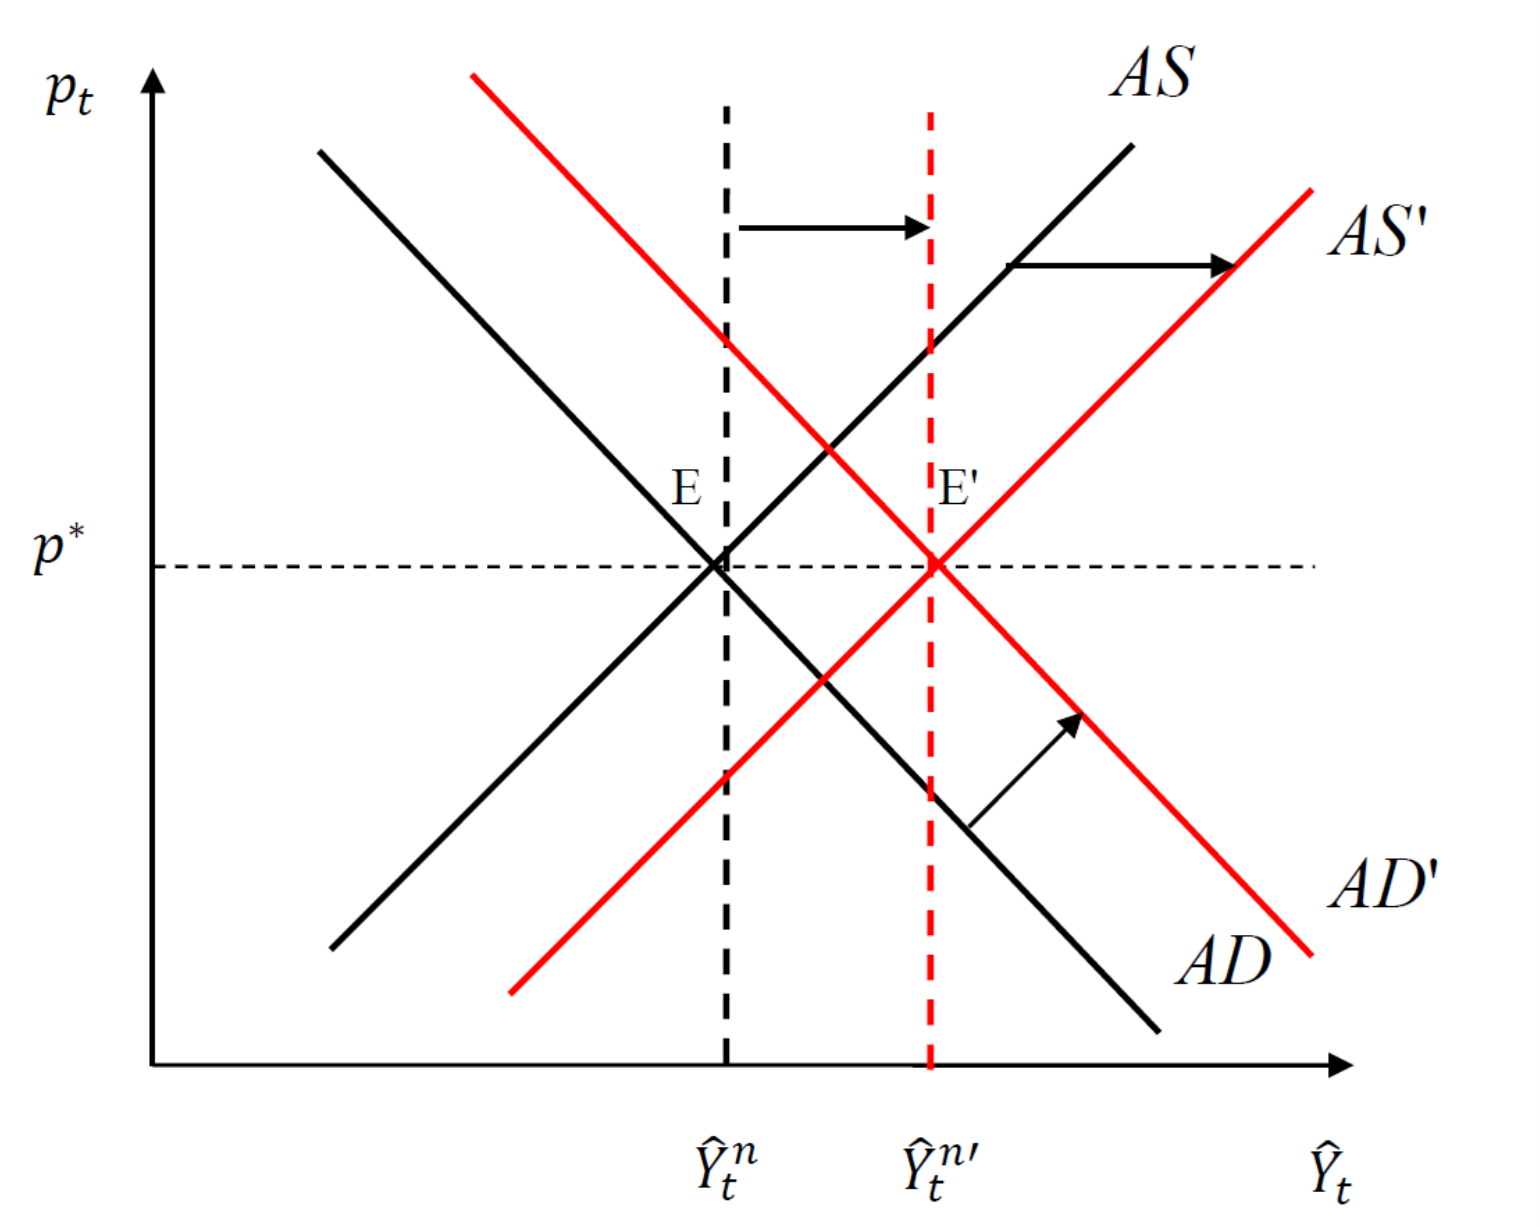
\includegraphics[width=\linewidth]{Figures/Figure5.png}
    \label{FigureASAD3}
\end{figure}
\end{column}

\end{columns}
\end{frame}

% --- SLIDE 2: Equilibrium and Policy Implications ---
\begin{frame}[label=PermProdPolicy]{Policy Response}
\small

\textbf{Equilibrium $E'$:}
\begin{itemize}
    \item The $AD$ curve shifts exactly to intersect the new $AS$ curve at $E'$.
    \item Result: Output increases to the new natural level ($\hat{Y}_t = \hat{Y}_t^n$), coinciding with the efficient level.
    \item Prices remain stable ($p_t = p^{\ast}$) without intervention.
\end{itemize}

\textbf{Why no policy intervention?}
\begin{itemize}
    \item \textbf{Real Rate Stability:} A permanent gain in productivity does \emph{not} change the frictionless real interest rate ($r^e_t$), as shown in \eqref{efficientr}.
    \item Since $\hat{Y}_{t}^{n}$ and $\hat{Y}_{t+1}^{n}$ increase in the same proportion, the "growth rate" of natural output is unchanged.
\end{itemize}

\textbf{Conclusion:}
\begin{itemize}
    \item The economy achieves price stability and closes the output gap automatically.
\end{itemize}

\end{frame}

% --- SLIDE 1: Productivity News/Optimism (Setup + Figure) ---
\begin{frame}[label=NewsShockSetup]{Optimism or "News" on Future Productivity}
\small
\begin{columns}[c]

\begin{column}{0.4\textwidth}
\small
\textbf{Scenario:}
\begin{itemize}
    \item Expected increase in future productivity: $\hat{A}_{t+1} \uparrow$ (but $\hat{A}_t$ remains constant).
\end{itemize}
\vspace{0.2cm}

\textbf{Implications:}
\begin{itemize}
    \item \textbf{AS unchanged}: Current productivity is unchanged, so current marginal costs are unaffected.
    \item \textbf{AD shifts upwards to AD'}: Households anticipate higher future income ($\hat{Y}_{t+1}^n \uparrow$). To smooth consumption, they increase demand today.
 
\end{itemize}
\end{column}

\begin{column}{0.58\textwidth}
\centering
\begin{figure}
    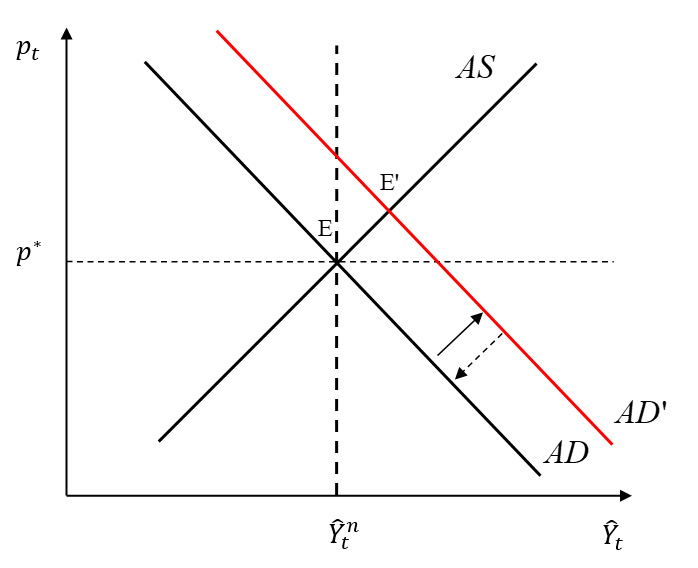
\includegraphics[width=\linewidth]{Figures/Figure6.png}
    \label{FigureASAD4}
\end{figure}
\end{column}

\end{columns}
\end{frame}

% --- SLIDE 2: Policy Response to Optimism ---
\begin{frame}[label=NewsShockPolicy]{Policy Response}
\small

\textbf{The New Equilibrium ($E'$):}
\begin{itemize}
    \item Intersection of the original $AS$ and the new $AD'$.
    \item Output expands beyond the natural level ($\hat{Y}_t > \hat{Y}_t^n$), and the efficient level.
    \item \textbf{Inflationary:} High demand drives up real wages and marginal costs, forcing firms to raise prices.
\end{itemize}

Restoring price stability and closing output gap in \textbf{equilibrium ($E''$):}
\begin{itemize}
    \item The central bank must \textbf{raise the nominal interest rate}.
    \item This restricts demand, shifting the $AD$ curve back down to the initial point $E$.
\end{itemize}

\textbf{Wicksellian Interpretation:}
\begin{itemize}
    \item Because the frictionless real rate ($r^e_t$) has increased, as in \eqref{efficientr}, the policy rate should follow.
\end{itemize}

\end{frame}
\begin{frame}{Productivity Shocks — Key Takeaways}

\begin{itemize}
\item Monetary policy can always stabilize \textbf{both inflation and the output gap} under productivity shocks.
\vspace{0.3cm}
\item The \textbf{direction} of the interest rate movement depends on the nature of the shock:
\begin{itemize}
\item \textbf{Temporary positive shock}: policy should be expansionary (rate cut).
\item \textbf{Permanent productivity improvement}: policy unchanged.
\item \textbf{Expected future productivity growth}: policy should tighten (rate hike).
\end{itemize}
\vspace{0.3cm}
\item The \textbf{Wicksellian natural rate} is the benchmark: the policy rate must adjust in the same direction as changes in $r^e_t$.
\end{itemize}

\end{frame}
%==================================================

\section{Markup Shock}
%==================================================
% SLIDE 1 — Markup Shock (Setup)
%==================================================
\begin{frame}[label=MarkupSetup]{Markup Shock}
\small
\begin{columns}[c]

% LEFT COLUMN
\begin{column}{0.42\textwidth}
\textbf{Scenario}
\begin{itemize}
\item Temporary increase in the markup: $\hat{\mu}_{t} \uparrow$.
\end{itemize}

\vspace{0.15cm}
\textbf{Implications:}
\begin{itemize}
\item $\hat{Y}^{e}_{t}$ fixed; $\hat{Y}^{n}_{t}\downarrow$, see \eqref{Efficient1} \& \eqref{Natural1}.
\item \textbf{AS shifts upwards to AS'}: firms raise prices driven by the cost-push shock.
\item \textbf{AD unchanged}, adjustment along the schedule due to higher real rate reducing consumption.
\item \textbf{Stagflation}: In equilibrium E' stagnation and inflation. Output falls and prices increase.
\end{itemize}
\end{column}

% RIGHT COLUMN
\begin{column}{0.56\textwidth}
\centering
\begin{figure}
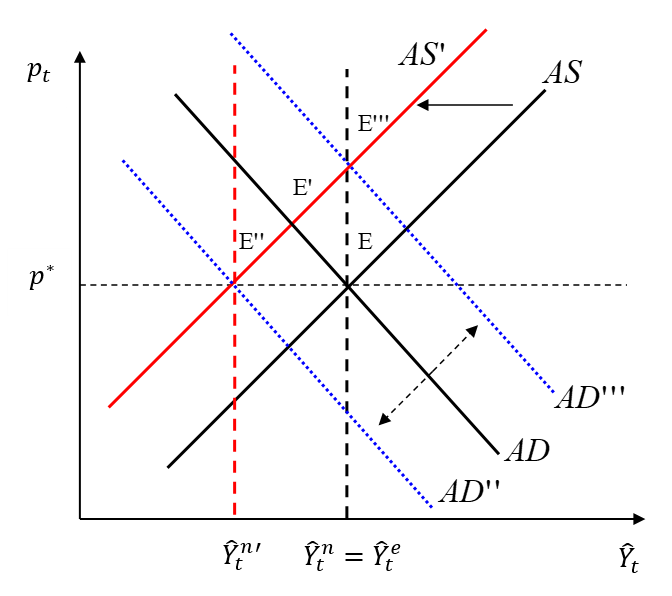
\includegraphics[width=\linewidth]{Figures/Figure7.png}
\end{figure}
\end{column}

\end{columns}
\end{frame}

%==================================================
% SLIDE 2 — Policy Trade-Off (Aligned Columns)
%==================================================
\begin{frame}[label=MarkupPolicy]{Stagflation: Policy Trade-Off}
\small

A markup shock creates a direct policy conflict: stabilizing prices and maintaining efficient output cannot be achieved simultaneously.

\vspace{0.2cm}

\begin{columns}[t] % <---- top alignment ensures equal starting height

% LEFT COLUMN
\begin{column}{0.40\textwidth}
\textbf{Option A: Stabilize Prices ($E''$)}
\begin{itemize}
\item Raise nominal interest rate ($i_t \uparrow$).
\item Aggregate demand shifts down ($AD \rightarrow AD''$).
\item Inflation returns to target, but output contracts further.
\end{itemize}
\end{column}

% RIGHT COLUMN
\begin{column}{0.40\textwidth}
\textbf{Option B: Reach Efficient Output ($E'''$)}
\begin{itemize}
\item Lower nominal interest rate ($i_t \downarrow$).
\item Aggregate demand shifts up ($AD \rightarrow AD'''$).
\item Output returns to $\hat{Y}^e_t$, but inflation rises.
\end{itemize}
\end{column}

\end{columns}

\vspace{0.2cm}

\textbf{Wicksellian implication:}
\begin{itemize}
\item Frictionless real rate $r_t^e$ is unchanged, so it \textbf{no longer guides optimal policy}.
\end{itemize}

\end{frame}
%=================================================
\section{Fiscal (Public Spending) Shock}
% --- SLIDE 1: Public Spending Shock (Setup + Figure) ---
\begin{frame}[label=GovShockSetup]{Temporary Public Spending Shock}
\small
\begin{columns}[c]

\begin{column}{0.37\textwidth}
\small
\textbf{Scenario:} A temporary increase in public spending at $t$: ($\hat{G}_t \uparrow$).
\\ \vspace{0.3cm}
\textbf{Implications:}
\begin{itemize}
    \item $\hat{Y}^{e}_{t}\uparrow$; $\hat{Y}^{n}_{t}\uparrow$, see \eqref{Efficient1} \& \eqref{Natural1}.
    \item \textbf{AD shifts upward to AD'}: Higher $\hat{G}_t$ directly expands demand for given consumption.
    \item \textbf{AS shifts downward to AS'}: Higher natural output $\hat{Y}_t^{n}$ shifts AS downward.
\end{itemize}
\end{column}

\begin{column}{0.6\textwidth}
\centering
% Wrapped in figure to allow proper labeling if caption is added later
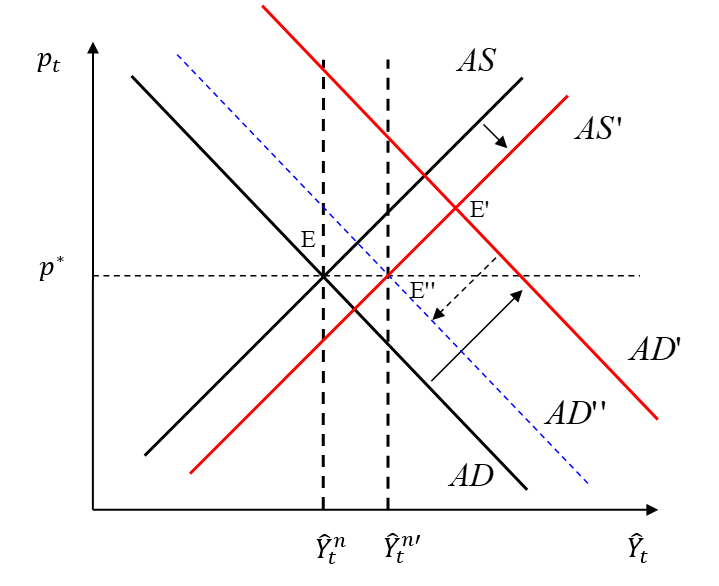
\includegraphics[width=\linewidth]{Figures/Figure8.png}
\label{FigureASAD6} 
\end{column}

\end{columns}
\end{frame}

% --- SLIDE 2: Policy Response (E -> E' -> E'') ---
\begin{frame}[label=GovShockPolicy]{Policy Response}
\small

\textbf{Equilibrium ($E'$):}
\begin{itemize}
    \item $AD$ shift dominates the $AS$ shift: Prices rise and output expands.
    \item Equations \eqref{ADsimple}, \eqref{ASsimple} and \eqref{Natural1} imply a \textbf{positive output gap} unless $\eta=0$.
\end{itemize}

\textbf{Restoring the efficient equilibrium ($E''$):}
\begin{itemize}
    \item A higher nominal rate $\hat{\imath}_t$ shifts $AD'$ downward to $AD''$.
    \item The new intersection $E''$ features both $p_t = p^{\ast}$ and $\hat{Y}_t = \hat{Y}^n_t = \hat{Y}^e_t$.
\end{itemize}

\textbf{Wicksell interpretation:}
\begin{itemize}
    \item Because the frictionless real rate ($r^e_t$) has increased, the policy rate should follow.
    \item \textbf{Note:} If $\eta=0$, $r_t^e$ remains constant; AD and AS adjust proportionally, automatically closing the output gap and keeping prices stable without policy intervention.
\end{itemize}
\end{frame}

%==================================================
\section{Preference Shock}
%==================================================
% SLIDE 1 — Preference Shock: Setup
%==================================================
\begin{frame}[label=PrefShockSetup]{Preference Shock}
\small

\textbf{Scenario:} Households become more patient: $\hat{\xi}_t \downarrow$ or $\hat{\xi}_{t+1} \uparrow$.
\\
\vspace{0.3cm}
\textbf{Implications:}
\begin{itemize}
    \item Households more patient today → want to save more.
    \item Frictionless equilibrium: $r^e_t \downarrow$, see \eqref{efficientr} to clear excess saving since efficient output unchanged ($\hat{Y}^e_t$).
    \item With sticky prices: $AD$ shifts downward → $\hat{Y}_t \downarrow$, $p_t \downarrow$ (along the unchanged $AS$).
    \item Output falls below efficient level.
    \item Prices decline along $AS$ curve.
\end{itemize}

\end{frame}

%==================================================
% SLIDE 2 — Preference Shock: Policy Response
%==================================================
\begin{frame}[label=PrefShockPolicy]{Preference Shock — Policy Response}
\small

\textbf{Monetary Policy Response:}
\begin{itemize}
    \item Cut nominal interest rate $\hat{\imath}_t$ proportionally to the fall in $r^e_t$.
    \item $AD$ shifts back upward → restores $p_t = p^{\ast}$ and closes output gap.
\end{itemize}

\textbf{Key Insights:}
\begin{itemize}
    \item Preference shocks affect only $AD$, similar to expected productivity news.
    \item Movements in the frictionless rate $r^e_t$ guides policy adjustment.
\end{itemize}
\textbf{Liquidity trap preview:}
\begin{itemize}
    \item Large fall in $\hat{\xi}_t$ can push $r^e_t < 0$; if zero lower bound binds, stabilizing prices and output simultaneously may be infeasible (see Chapter 9).
\end{itemize}

\end{frame}

%==================================================
\section{Disanchoring of Long-Run Price Expectations}
% --- SLIDE 1: The Modified Framework (Equations) ---
\begin{frame}[label=ExpEquations]{Disanchoring Expectations}
\small

\textbf{Assumption:}
We relax the assumption that long-run price expectations are rigidly anchored at $p^{\ast}$. We distinguish between:
\begin{itemize}
    \item $\bm{E_{t}^{d}p_{t+1}}$: Consumers' expectations (affects Demand).
    \item $\bm{E_{t}^{s}p_{t+1}}$: Firms' expectations (affects Supply).
\end{itemize}
\vspace{0.3cm}

\textbf{Modified AD Equation (Consumer Expectations):}
\begin{equation*}
\hat{Y}_{t}-\hat{Y}_{t}^{e}=-\sigma \left( \hat{\imath}_{t}-(E_{t}^{d}p_{t+1}-p_{t})-r_{t}^{e}\right)
\end{equation*}

\textbf{Modified AS Equation (Firm Expectations):}
\begin{equation*}
p_{t}=\frac{1}{1+\beta }p^{\ast }+\frac{\kappa }{1+\beta }(\hat{Y}_{t}-\hat{Y}_{t}^{n})+\frac{\beta }{1+\beta }E_{t}^{s}p_{t+1}
\end{equation*}

\end{frame}

% --- SLIDE 2: Consumer Expectations (Demand Shift) ---
\begin{frame}[label=ExpDemand]{Disanchoring: Consumer Inflation Expectations}
\small

\textbf{Scenario:}
\begin{itemize}
    \item Consumers adjust long-run price expectations downward ($E_{t}^{d}p_{t+1} \downarrow$).
\end{itemize}

\textbf{Implications:}
\begin{itemize}
    \item Lower expected inflation leads to an increase in the real interest rate (for a given nominal $i_t$).
    \item Households increase savings and postpone consumption.
    \item The $AD$ curve shifts \textbf{downward} from the initial equilibrium.
    \item Output and prices both fall ($\hat{Y}_t \downarrow, p_t \downarrow$) along the unchanged AS leading to a \textbf{potential deflationary spiral.}
\end{itemize}
\vspace{0.3em}
\textbf{Policy:}
\begin{itemize}
    \item The central bank should consider lowering the nominal rate to stimulate demand and shift $AD$ back.
\end{itemize}
\end{frame}
% --- SLIDE 3: Firm Expectations (Supply Shift) ---
\begin{frame}[label=ExpSupply]{Disanchoring: Firm Inflation Expectations}
\small

\textbf{Scenario:}
\begin{itemize}
    \item Firms anticipate a future increase in the price level ($E_{t}^{s}p_{t+1} \uparrow$).
\end{itemize}

\textbf{Implications:}
\begin{itemize}
    \item Strategic pricing: firms incorporate higher future prices into current decisions.
    \item The $AS$ curve shifts \textbf{upward} from the initial equilibrium.
    \item Current prices rise while output contracts ($\hat{Y}_t \downarrow, p_t \uparrow$), leading to a \textbf{potential inflationary spiral.}
\end{itemize}
\vspace{0.3em}
\textbf{Policy:}
\begin{itemize}
    \item \textbf{Stagflation:} The economy faces a trade-off (similar to a Markup Shock).
\end{itemize}
\end{frame}

%==================================================
\section{Key Takeaways}

\begin{frame}{Main Takeaways}
\small
\begin{itemize}
  \item With \textbf{efficient shocks} (productivity, public spending, preference): 
  aligning the policy-controlled real rate 
  \[
      \hat{\imath}_t - (p^{*} - p_t),
  \]
  with the efficient real rate \(r_t^{e}\) delivers price stability \emph{and} closes the efficient output gap.
  
  \vspace{0.35cm}
  
  \item With \textbf{inefficient shocks} (e.g.\ markup shocks): 
  the efficient real rate \(r_t^{e}\) is no longer an appropriate guide. 
  Policymakers face a \emph{trade-off} between stabilizing inflation and closing the output gap.
  
  \vspace{0.35cm}
  
  \item \textbf{Expectations matter}: 
  a disanchoring of long-run price expectations \(E_t p_{t+1}\) can be destabilizing. 
  This reinforces the need for monetary policy to firmly anchor expectations.
\end{itemize}
\end{frame}

%==================================================
\appendix
\section{Appendix}
%==================================================
\begin{frame}{Shock-by-Shock Logic}

    % 1. Increase vertical spacing between rows for readability
    \renewcommand{\arraystretch}{1.3} 
    % 2. Reduce horizontal padding between columns (default is 6pt)
    \setlength{\tabcolsep}{3pt} 

    \begin{center}
    % 3. Resizebox forces the table to fit the text width exactly
    \resizebox{\textwidth}{!}{%
        \begin{tabular}{lcccccc}
            \toprule
            \textbf{Shock} & \textbf{AD} & \textbf{AS} & $\bm{r^e_t}$ & \textbf{Prices} & \textbf{Output Gap} & \textbf{Policy} $\bm{i_t}$ \\
            \midrule
            Productivity (temp $\,\hat{A}_t \uparrow\,$) & $\cdot$ & $\downarrow$ & $\downarrow$ & $\downarrow$ & - & $\downarrow$ \\
            
            Productivity (perm $\,\hat{A}_t, \hat{A}_{t+1} \uparrow\,$) & $\uparrow$ & $\downarrow$ & $\cdot$ & $\cdot$ & $\cdot$ & $\cdot$ \\
            
            Productivity news ($\,\hat{A}_{t+1} \uparrow\,$) & $\uparrow$ & $\cdot$ & $\uparrow$ & $\uparrow$ & + & $\uparrow$ \\
            
            Markup ($\,\hat{\mu}_t \uparrow\,$) & $\cdot$ & $\uparrow$ & $\cdot$ & $\uparrow$ & - & Trade-off \\
            
            Public spending (temp $\,\hat{G}_t \uparrow\,$) & $\uparrow$ & $\downarrow$ & $\uparrow$ & $\uparrow$ & + & $\uparrow$ \\
            
            Preferences ($\,\hat{\xi}_t \downarrow\,$) & $\downarrow$ & $\cdot$ & $\downarrow$ & $\downarrow$ & - & $\downarrow$ \\
            \bottomrule
        \end{tabular}%
    } % End of resizebox
    \end{center}

    \vspace{0.2cm}
    \scriptsize \textit{Note:} Dots indicate “no change”. Signs reflect movements from the \emph{initial} equilibrium.

\end{frame}
\begin{frame}{Parameter and Variable Map}
    \centering
    \small
    
    % --- PART 1: STRUCTURAL PARAMETERS ---
    \centering{\textbf{Parameters}}
    \vspace{0.2em}
    
    % Using 4 columns (Sym | Desc || Sym | Desc) to save vertical space
    \renewcommand{\arraystretch}{1.2}
    \begin{tabular}{r l @{\hspace{1cm}} r l}
        \toprule
        $\sigma > 0$ & IES & $\eta > 0$ & Inverse Frisch elasticity \\
        $\beta \in (0,1)$ & Discount factor & $\kappa > 0$ & Slope of the NKPC \\
        \bottomrule
    \end{tabular}

    \vspace{1.5em} % Visual separation between the two tables

    % --- PART 2: VARIABLES & SHOCKS ---
    \centering{\textbf{Variables \& Shocks}}
    \vspace{0.2em}
    
    % Standard 2-column table for the list of variables
    \renewcommand{\arraystretch}{1.3} % More breathing room for the hats/superscripts
    \begin{tabular}{r l}
        \toprule
        $\hat{Y}_t, \hat{Y}^n_t, \hat{Y}^e_t$ & Log-deviation of Output (Actual, Natural, Efficient) \\
        $\hat{\imath}_t, r^e_t$ & Nominal Policy Rate vs. Wicksellian Real Rate \\
        $p^{\ast}$ & Long-run Price Anchor \\
        \addlinespace % Adds a subtle gap
        $\hat{G}_t, \hat{A}_t$ & Public Spending \& Productivity Shocks \\
        $\hat{\mu}_t, \hat{\xi}_t$ & Markup \& Preference Shocks \\
        \bottomrule
    \end{tabular}
    
\end{frame}
%
\end{document}
